\documentclass[
    10pt, % Set the default font size, options include: 8pt, 9pt, 10pt, 11pt, 12pt, 14pt, 17pt, 20pt
    %
    aspectratio=169, % Uncomment to set the aspect ratio to a 16:9 ratio which matches the aspect ratio of 1080p and 4K screens and projectors
]{beamer}
\usepackage{transparent}
\usepackage{booktabs} 
\usepackage{tabularx}
\usepackage{makecell}
\beamertemplatenavigationsymbolsempty
%\usepackage{appendixnumberbeamer} %If you want a separate slide counter for your appendix

%%% To add citations
\usepackage[
    style=nature,
    sorting=none,
    isbn=false,
    url=false,
    doi=true,
    eprint=false,
    date=year,
    maxnames=3,
    minnames=2
]{biblatex}
\addbibresource{bibliography.bib}
\renewcommand*{\bibfont}{\normalfont\fontsize{5}{5}\selectfont}
\usepackage{algorithm}
\usepackage{algpseudocode}
\usepackage{lipsum}
\usepackage{hyperref}
%%% Customize Theme %%%%%%%%%%%%%%%%%%%%%%
\usetheme[width=3.8em]{Goettingen} % Best one with a sidebar, IMO. But it's worth exploring other Beamer Themes, too.


\addtobeamertemplate{sidebar right}{}{ 
 \hspace*{.5em}{\transparent{0.5} 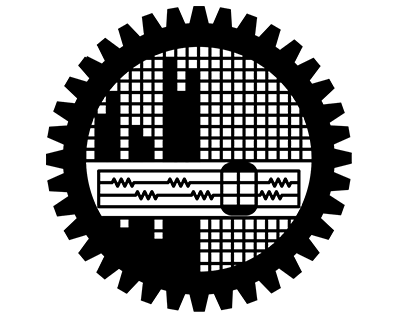
\includegraphics[width = 0.131\textwidth]{buet logo 4.png}}%
}

%----------------------------------------------------------
%           Colour Setup
%----------------------------------------------------------

%fg = font color
%bg = background color

% ! WARNING ! : Many colors are linked to multiple attributes, so changing one color can have unexpected changes!

% If you want to tweak the shading of orange and red, tweak the below 2 lines:
\definecolor{myRed}{RGB}{163, 10, 53}
\definecolor{myOrange}{RGB}{254, 195, 26}
\setbeamertemplate{sidebar canvas right}[vertical shading][top=myRed, middle=myRed!85, bottom=myRed]
% Bottom right hand color
\setbeamercolor*{structure}{bg=myOrange,fg=myRed}

\setbeamercolor*{palette primary}{use=structure,fg=white,bg=structure.fg} %?
\setbeamercolor*{palette secondary}{use=structure,fg=myRed,bg=myOrange}
    %bottom left of footer & bar between title & top bubbles
\setbeamercolor*{palette tertiary}{use=structure,fg=white,bg=myRed} 

\setbeamercolor{frametitle}{bg=myRed,fg=white} %title of each slide

\setbeamercolor*{titlelike}{parent=palette primary} %?

%%% Edits ONLY the TOC slide %%%
\setbeamercolor{section in toc}{fg=black}
\setbeamercolor{subsection in toc}{fg=black}

%%% Block Colors %%%
% Standard block %
    \setbeamercolor{block title}{bg=myOrange, fg=white}
    \setbeamercolor{block body}{bg=myOrange!20}

% Alerted block % If you want to customize it's color
    %\setbeamercolor{block title alerted}{bg=cyan, fg=white}
    %\setbeamercolor{block body alerted}{bg=cyan!10}

% Example block % If you want to customize it's color
    %\setbeamercolor{block title example}{bg=cyan, fg=white}
    %\setbeamercolor{block body example}{bg=cyan!10}

\setbeamercolor{title in sidebar}{fg=white!75}
\setbeamercolor{author in sidebar}{fg=white!50}
\setbeamercolor{palette sidebar secondary}{fg=myRed,bg=white!80}
\setbeamercolor{subsection in sidebar}{fg=myRed,bg=white!80}
\setbeamercolor{section in sidebar shaded}{fg=white!75}
\setbeamercolor{subsection in sidebar shaded}{fg=white!75}
%---------------------------------------------------------
%	SELECT FONT THEME & FONTS
%---------------------------------------------------------

\usefonttheme{serif}
\usepackage{fontenc}
\usepackage{ebgaramond}

\setbeamerfont{frametitle}{size=\large}

%---------------------------------------------------------
%	SELECT OUTER THEME
%---------------------------------------------------------
% Outer themes change the overall layout of slides, such as: header and footer lines, sidebars and slide titles. Uncomment each theme in turn to see what changes it makes to your presentation.

\useoutertheme{default}

% This sets up the footer on each slide

\setbeamercolor{section in foot}{fg=white, bg=myRed}


\setbeamertemplate{footline}
{
 \hbox{%
  \begin{beamercolorbox}[wd=.12\paperwidth,ht=2.6ex,dp=2ex,center]{section in foot}%
    \usebeamerfont{section in foot}\insertshortauthor
  \end{beamercolorbox}%
  
  \begin{beamercolorbox}[wd=.65\paperwidth,ht=2.6ex,dp=2ex,center]{section in foot}%
    \usebeamerfont{section in foot} CSE 300 Presentation \text{    } \insertframenumber/\inserttotalframenumber
  \end{beamercolorbox}%
  
  \begin{beamercolorbox}[wd=.2\paperwidth,ht=2.6ex,dp=2ex,center]{section in foot}%
    \usebeamerfont{section in foot} 
  \end{beamercolorbox}}%

  \vskip0pt%
}



% Other Frames to consider...

%\useoutertheme{miniframes}
%\useoutertheme{infolines}
\useoutertheme{smoothbars}
%\useoutertheme{sidebar}
%\useoutertheme{split}
%\useoutertheme{shadow}
%\useoutertheme{tree}
%\useoutertheme{smoothtree}

%---------------------------------------------------------
%	PRESENTATION INFORMATION
%---------------------------------------------------------

\title[RB Tree]{Red Black Tree}
\subtitle{A Balanced Binary Tree}
\author[Kausar \and Sagor \and Souvik]{S.M. Kausar Parvej \and Sagor Chanda \and Souvik \\ 2005076    \and   2005071 \and  2005069 }

\date{\today}
\institute[BUET]{Bangladesh University of Engineering and Technology }

%%% This sets up the title page

\setbeamertemplate{title page}{
  \begin{minipage}[b][\paperheight]{\textwidth}
    \vfill%
    \ifx\inserttitle\@empty\else\usebeamertemplate*{title}\fi
    \ifx\insertsubtitle\@empty\else\usebeamertemplate*{subtitle}\fi
    \usebeamertemplate*{title separator}
    \ifx\beamer@shortauthor\@empty\else\usebeamertemplate*{author}\fi
    \ifx\insertdate\@empty\else\usebeamertemplate*{date}\fi
    \ifx\insertinstitute\@empty\else\usebeamertemplate*{institute}\fi
    \vfill
    \vspace*{1mm}
  \end{minipage}
    \raisebox{.1\paperheight}[1.7em][0em]{%
    \makebox[\paperwidth][c]{%
      \hspace*{-8.2em}\includegraphics[width=.883\paperwidth,height=1cm]{PHP.png}%
    }%
  }
}
\makeatother

%---------------------------------------------------------
%---------------------------------------------------------
%---------------------------------------------------------
\begin{document}

%---------------------------------------------------------
%	TITLE SLIDE
%---------------------------------------------------------
\section{}
\begin{frame}
	\titlepage % Output the title slide, automatically created using the text entered 
\end{frame}

%---------------------------------------------------------
%	TABLE OF CONTENTS SLIDE
%---------------------------------------------------------
% References sections and subsections, specified with the standard \section and \subsection commands. If you want to display all sections and subsections on one slide, just use \tableofcontents. If you want to just display each section one at a time (in subsequent slides) use \tableofcontents[pausesections].

%\tableofcontents



%---------------------------------------------------------
%	PRESENTATION BODY SLIDES
%---------------------------------------------------------

\section{Introduction}

\begin{frame}{Intro Slide}
    A Bullet List:
    \begin{itemize}
        \item Item One
        \item Cites \cite{Folch_Arribas-Bel_Koschinsky_Spielman_2016}
        \item More Cites \cite{singh_area_2003, spielman2020evaluating}
    \end{itemize}

\vspace{5em}

\href{https://www.youtube.com/watch?v=Unzc731iCUY}{Click Here for a Really Good Lecture on Presenting \& Speaking - Seriously}

\end{frame}

\section{Methods}

\begin{frame}{Methods Slide}
Bullets next to figure:

\begin{columns}
    \begin{column}{.4\textwidth}
        \begin{itemize}
            \item Method 1
            \item \textit{Special Method}
            \item \textbf{Important Method}
        \end{itemize}
        Maybe add a Formula?
        \begin{equation*}
                     y_i=\sum_{k=0}^K x_{ik} \circ \beta_ik+\varepsilon
                    \label{eq:svc}
                 \end{equation*}
    \end{column}
    \begin{column}{.6\textwidth}
        \begin{figure}
            \centering
            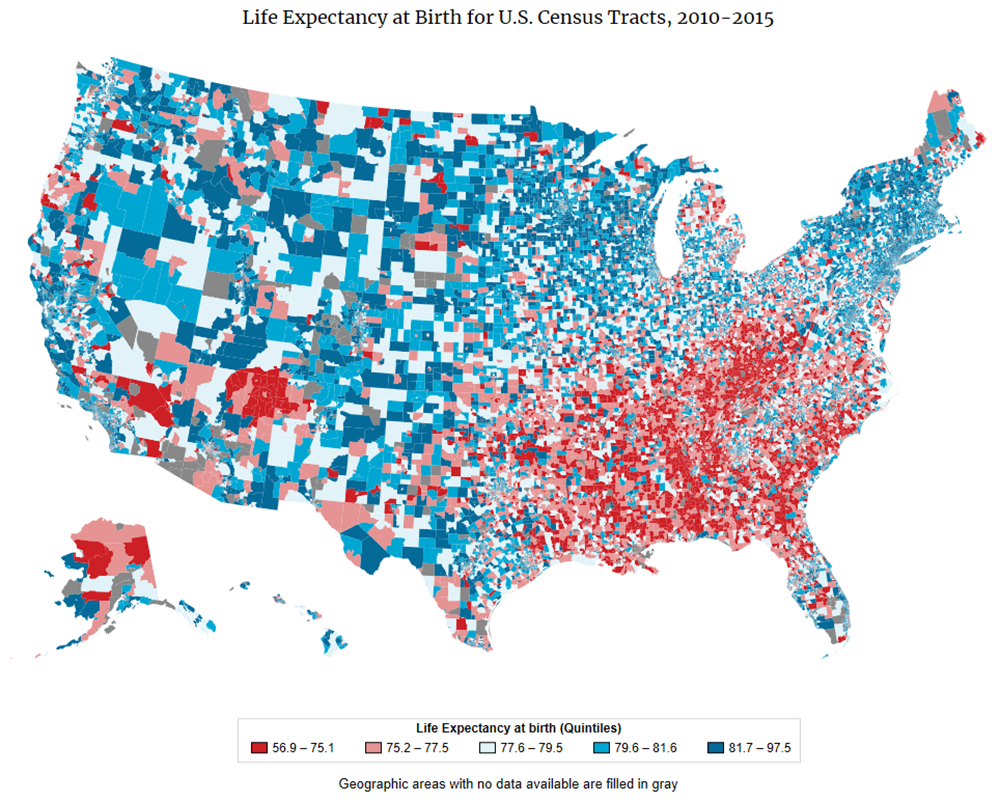
\includegraphics[scale=.3]{Images/LifeExpect.png}
            \caption{Motivating Figure}
            \label{fig:life-exp}
        \end{figure}
    \end{column}
\end{columns} 
\end{frame}

\section{Results}

\begin{frame}{Results Slide}
    \centering 
    Side-by-Side Images

    \begin{columns}
        \begin{column}{.45\textwidth}
            \begin{figure}
                \centering
                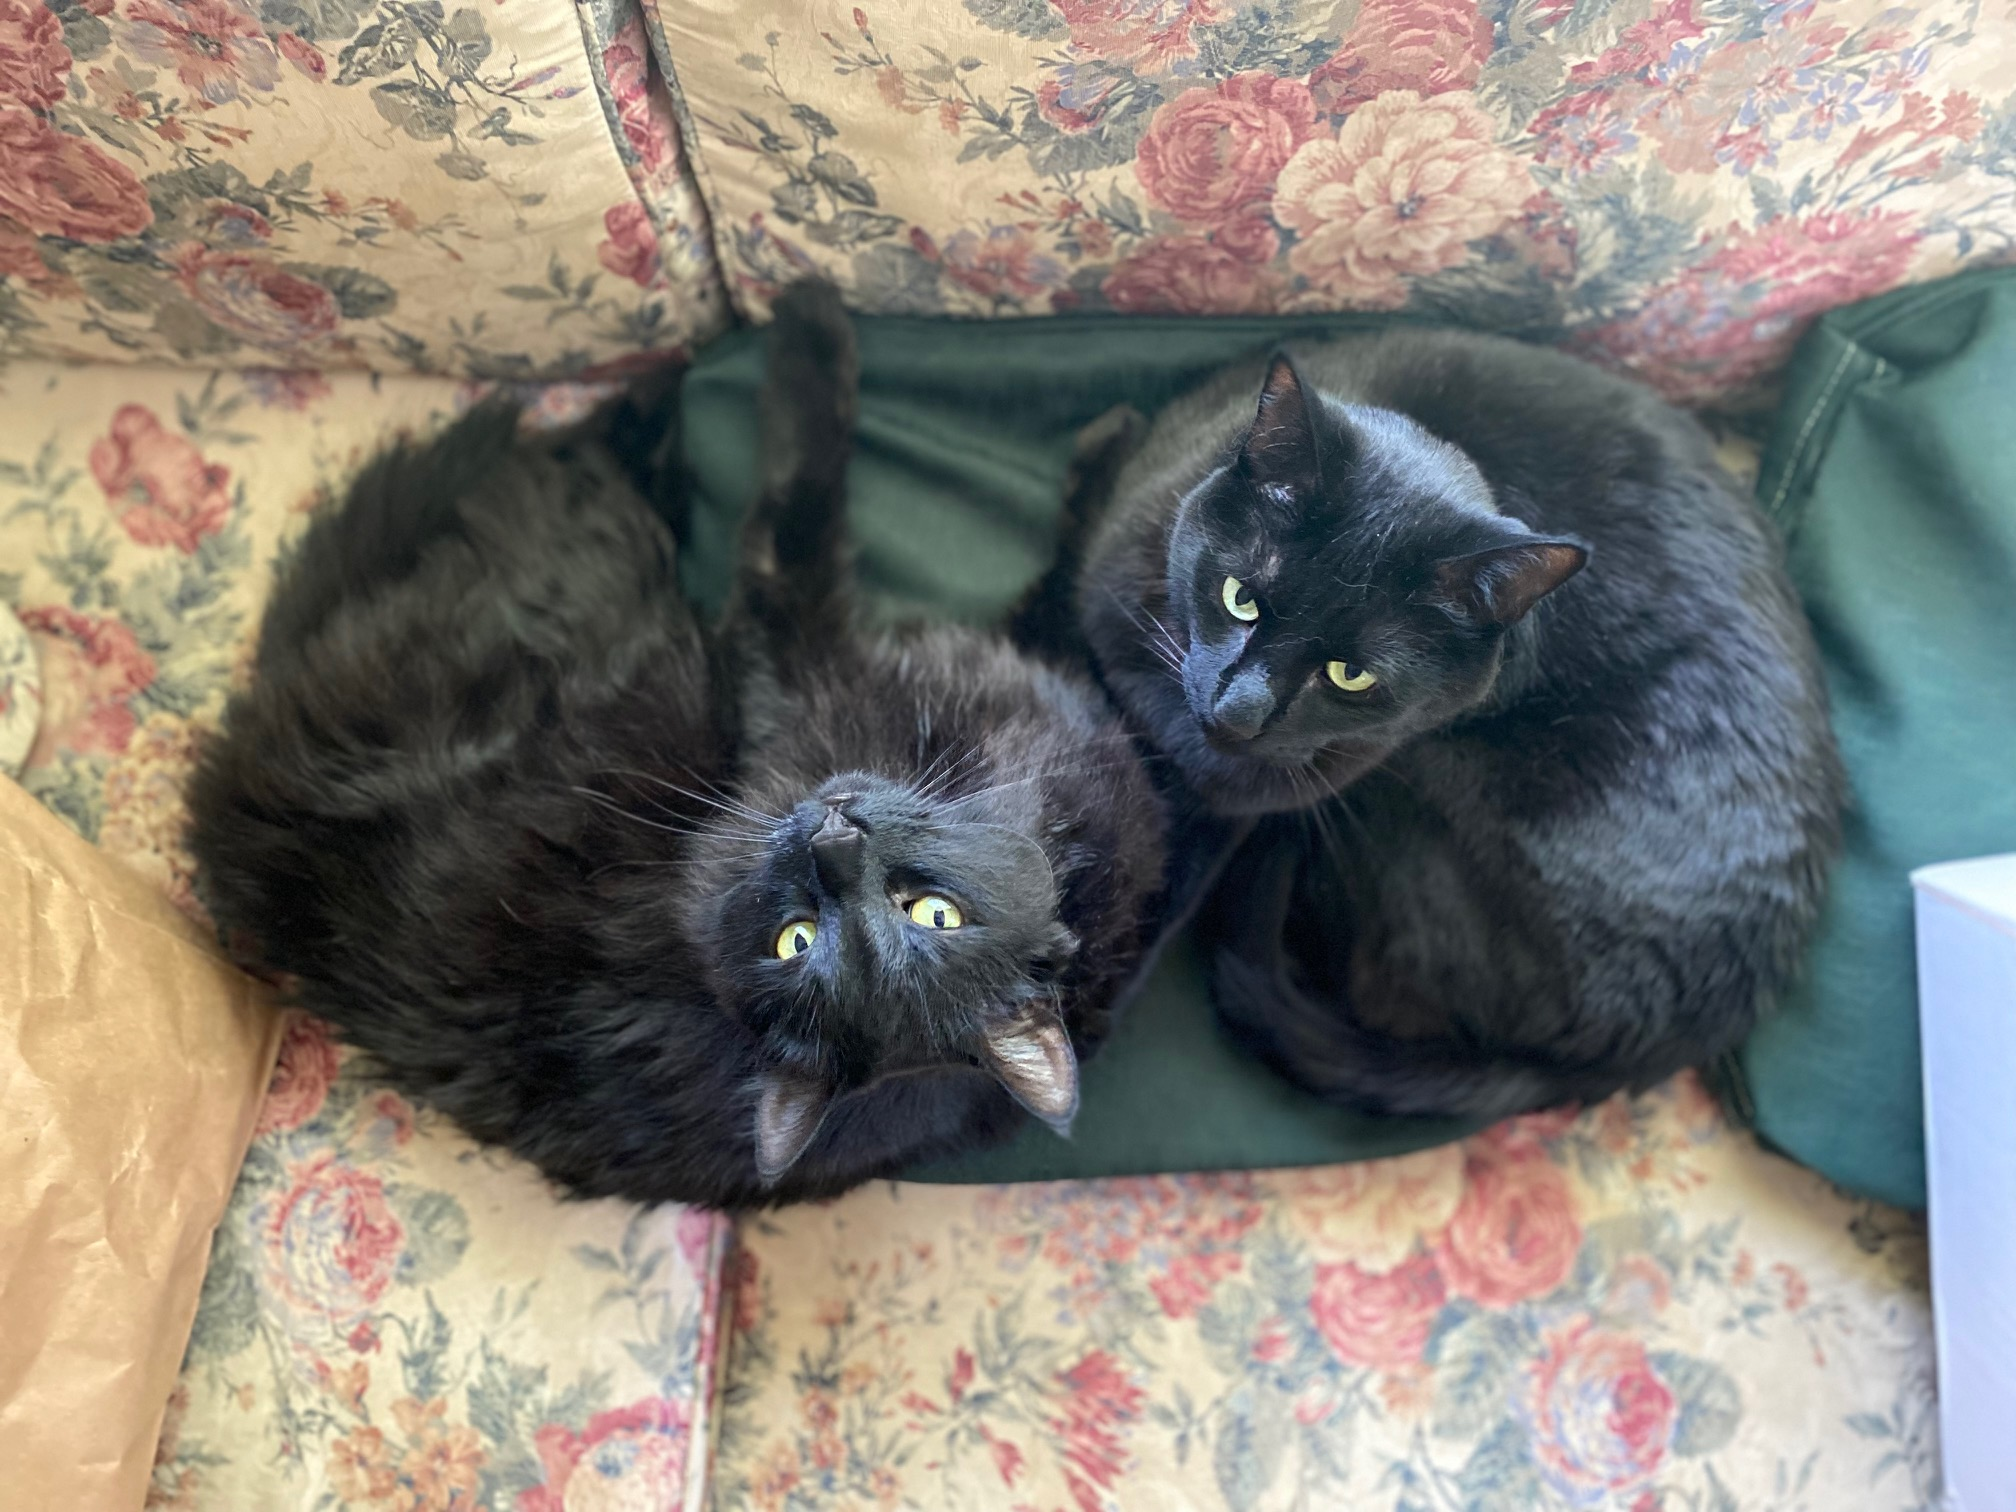
\includegraphics[scale=.08]{Images/kitties.jpg}
                \caption{Cats have no need for research}
                \label{fig:kitties}
            \end{figure}
        \end{column}
        \begin{column}{.45\textwidth}
            \begin{figure}
                \centering
                
\includegraphics[scale=.3]{Images/SadKeanu.jpg}
                \caption{Sad Keanu doesnt like your results.}
                \label{fig:keanu}
            \end{figure}
        \end{column}
    \end{columns}
\end{frame}

\section{Discussion}

\begin{frame}{Talk About How Awesome Your Work Is}

\textbf{Avoid having too much text on your slides}

\lipsum[1-2]
    
\end{frame}


%---------------------------------------------------------
%	REFERENCES
%---------------------------------------------------------

\begin{frame}[noframenumbering, allowframebreaks] 
        \frametitle{References}
        \printbibliography
\end{frame}


\begin{frame}[noframenumbering]
\label{Figure}
	\frametitle{Appendix - Algorithm}
        
        \begin{figure}[h!]
            \centering
            %\caption{}
            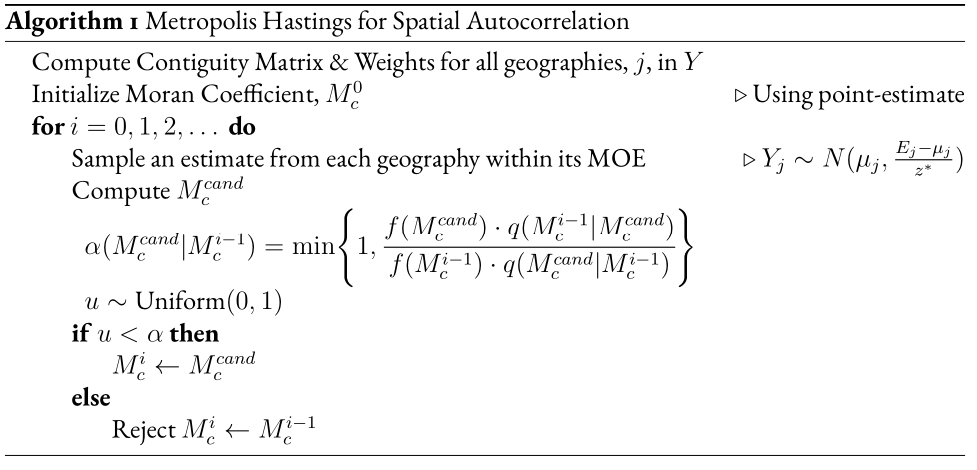
\includegraphics[angle=0, width=10cm]{Images/algo.png}
            %\label{fig}
        \end{figure}
\end{frame}


\end{document} 